%%%%%%%%%%%%%%%%%%%%%%%%%%%%%%%%%%%%%%%%%%%%%%%%%%%%%%%%%%%%%%%%%%%%%%%%%%%%%%%%
\chapter{Системотехническая часть}
%%%%%%%%%%%%%%%%%%%%%%%%%%%%%%%%%%%%%%%%%%%%%%%%%%%%%%%%%%%%%%%%%%%%%%%%%%%%%%%%

%%%%%%%%%%%%%%%%%%%%%%%%%%%%%%%%%%%%%%%%%%%%%%%%%%%%%%%%%%%%%%%%%%%%%%%%%%%%%%%%
\section{Анализ предметной области}
\subsection{Интерактивное обучение}
\subsection{Геймификация}
\subsection{Визуальное программирование}
\section{Обзор аналогов}
\subsection{Blockly}
\subsection{TRIK Studio}
\subsection{Дракон-схемы}
\section{Трансляция текстов программ}
\section{Форма Бэкуса-Наура}
\subsection{Компиляция}
\subsection{Интерпретация}
\section{API браузера}
\subsection{Очередь задач}
\subsection{Canvas}
%%%%%%%%%%%%%%%%%%%%%%%%%%%%%%%%%%%%%%%%%%%%%%%%%%%%%%%%%%%%%%%%%%%%%%%%%%%%%%%%

%\blindtext
%
%\begin{figure}[htbp]
%\centering
%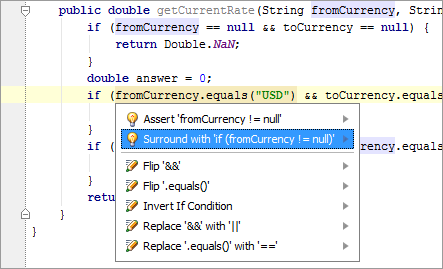
\includegraphics[width=\textwidth]{code_analysis_bugs.png}
%\caption{Рекомендации по проведению исследований в рамках диссертации}%
%\label{fig:how-to-do-research}
%\end{figure}
%
%\Blindtext
%
%\begin{table}
%% Для таблиц с multirow и multicol необходимо вручную указать сдвиг для caption
%\captionsetup{skip=5pt}
%\caption{Example}
%\centering
%\begin{tabular}{|r|c|c|c|c|c|c|}
%\hline
%            \multirow{2}{*}{}
%           & \multicolumn{2}{c|}{LLVM IR} 
%           & \multicolumn{2}{c|}{PS} 
%           & \multicolumn{2}{c|}{AI} \\ \cline{2-7}
%           & SAT    & UNSAT   & SAT    & UNSAT   & SAT    & UNSAT   \\ \hline
%beanstalkd & 356    & 252     & 360    & 161     & 360    & 247     \\ \hline
%clib       & 599    & 258     & 960    & 234     & 960    & 449     \\ \hline
%\end{tabular}
%\label{table:checkResults}
%\end{table}
%
%%%%%%%%%%%%%%%%%%%%%%%%%%%%%%%%%%%%%%%%%%%%%%%%%%%%%%%%%%%%%%%%%%%%%%%%%%%%%%%%%
%\section{bar}
%%%%%%%%%%%%%%%%%%%%%%%%%%%%%%%%%%%%%%%%%%%%%%%%%%%%%%%%%%%%%%%%%%%%%%%%%%%%%%%%%
%
%\blindtext
%It is of great importance that you use correct references in your dissertation.
%Resent studies show that it can increase the chances of successful defense
%by as much as 3,17 percent~\cite{russian, ANTLR, java-book}.
%
%\begin{table}[H]
%	\caption{Название таблицы}
%	\begin{center}
%		\begin{tabular}{|l|l|}
%			\hline
%			top left & top right\\ \hline
%			bot left & bot right\\ \hline
%		\end{tabular}
%		\label{tabular:tab_examp}
%	\end{center}
%\end{table}
%
%
%\Blindtext
